\section{Comparing the results of the user second journey}\label{section:results:comparison-second-journey}

This section shows another but a shorter comparison of the results between the three approaches explained in \ref{section:results:performance-measurement}. The journey of the client through the application is shown in figure \ref{fig:results:evaluation-second-path}. The client has to perform 17 steps throughout the application, which involves almost every available GraphQL query. In contrast to the first journey from \ref{section:results:comparison-first-journey}, the client uses an authenticated user to perform the test. The GraphQL \ac{API} request to retrieve the authenticated user has to be done by every micro-frontend individually, with the default approach with a separate cache.

\ifshowImages
\begin{figure}[H]
\centering
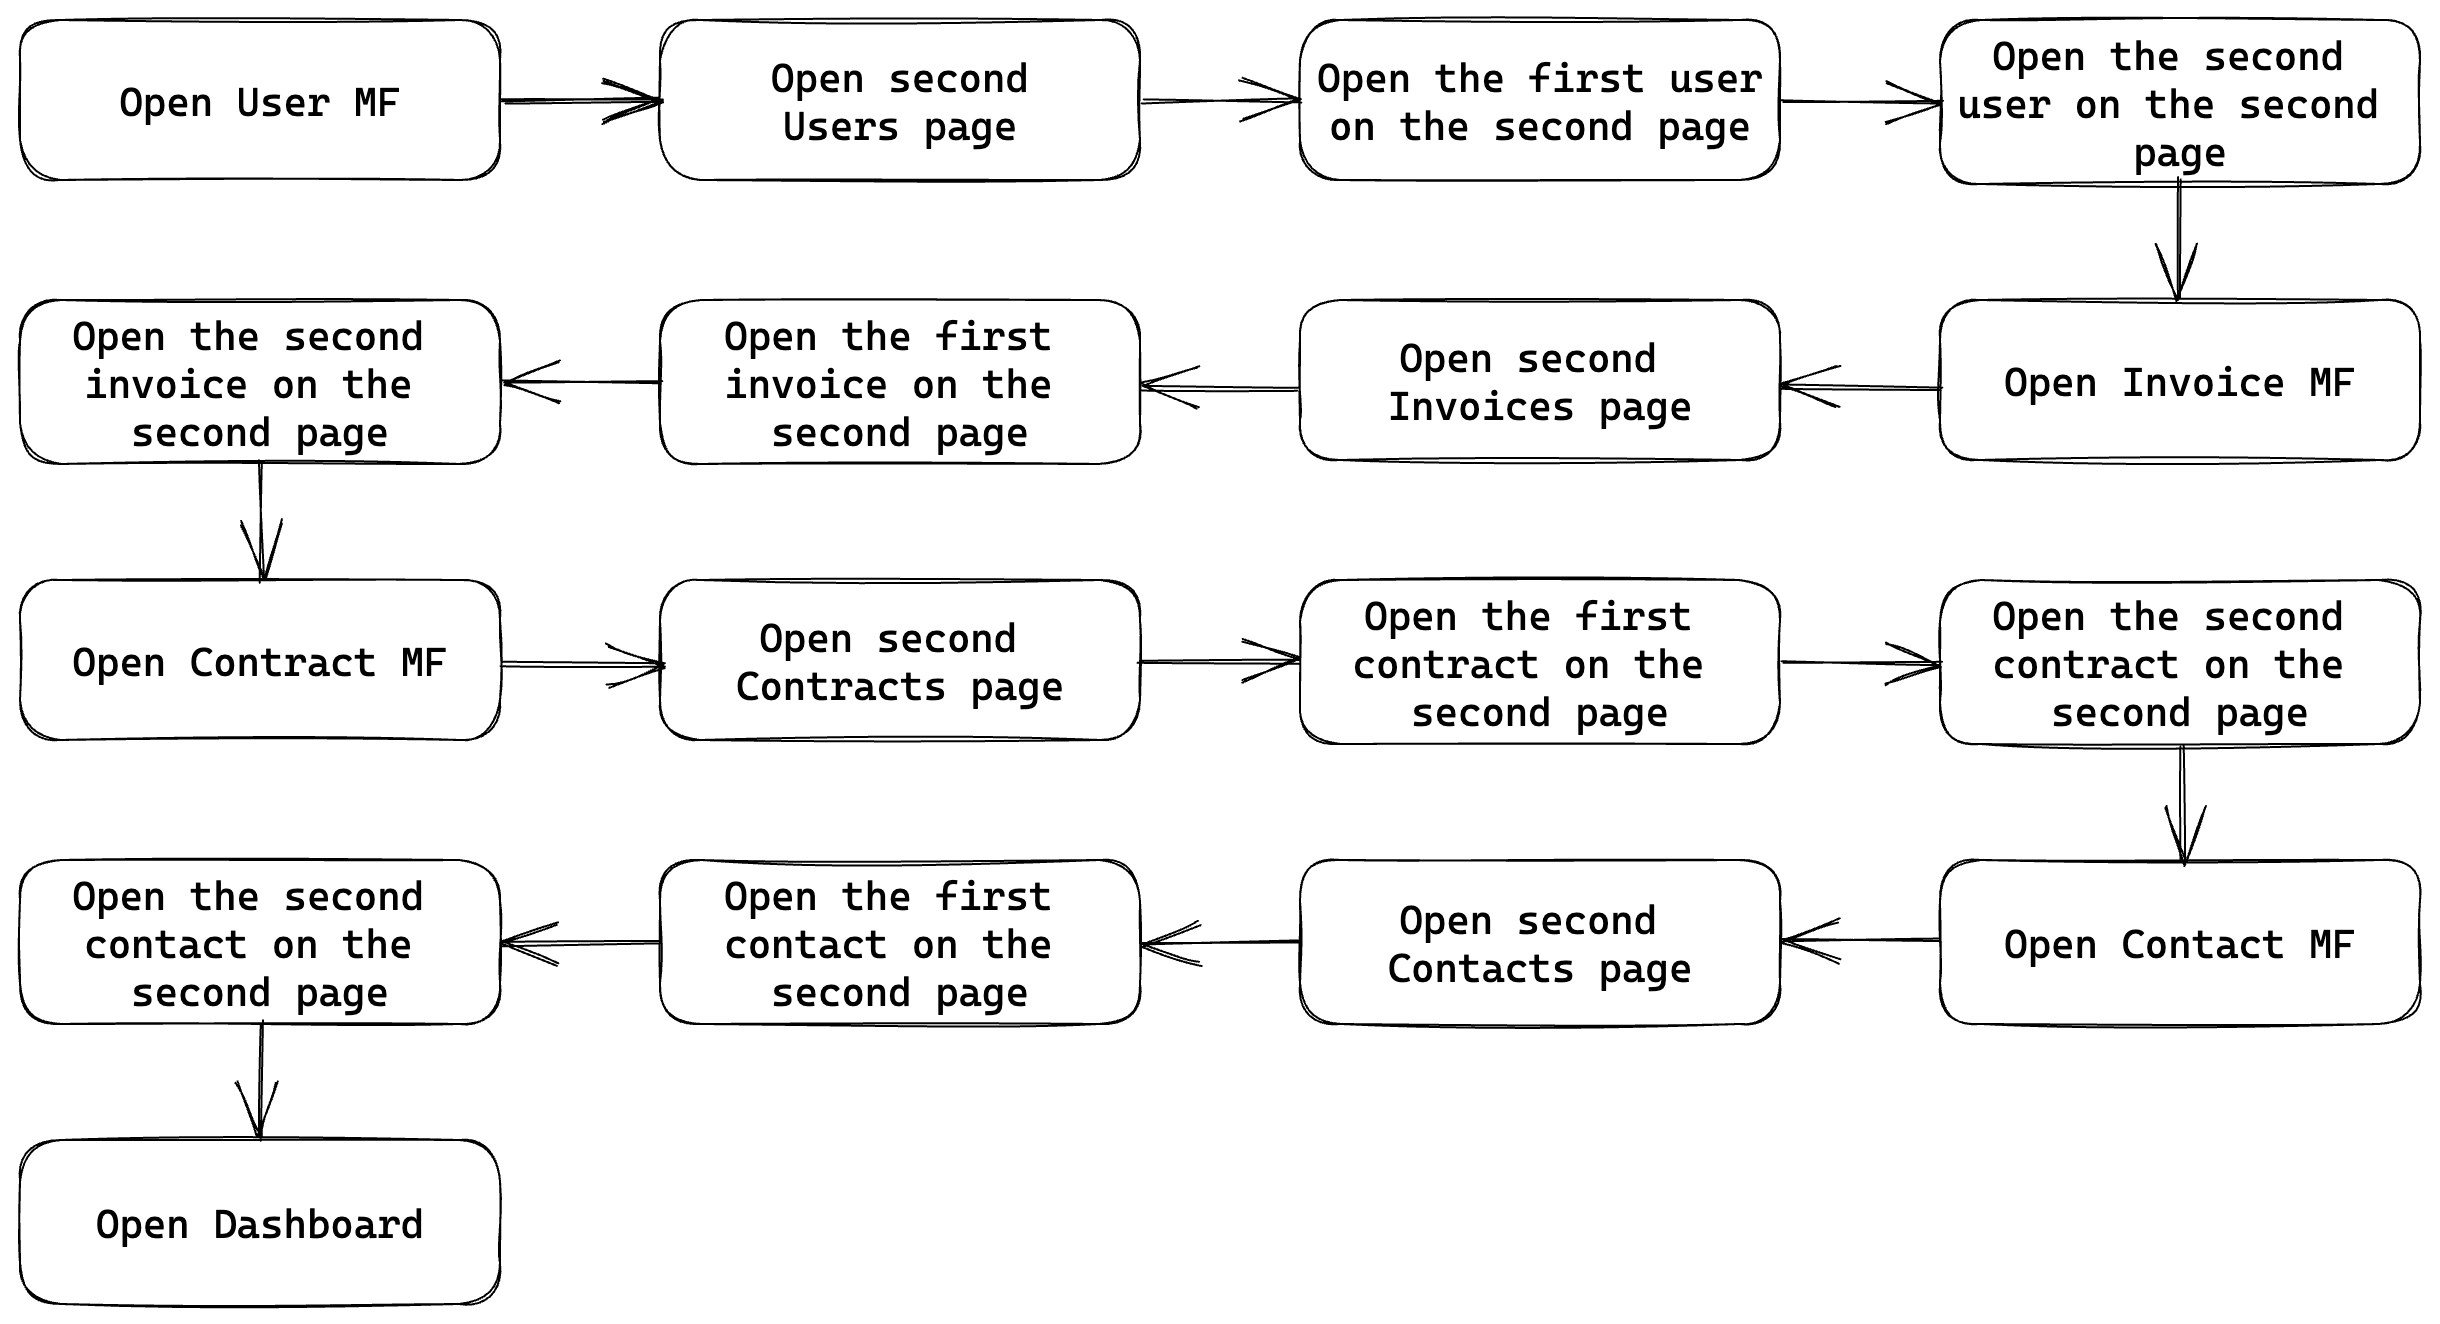
\includegraphics[width=1\linewidth]{images/results/evaluation-second-path.png}
\caption{The second user journey through the application to measure the performance of the micro-frontend architecture.}\label{fig:results:evaluation-second-path}
\end{figure}
\fi

\noindent The next sections compare the three different approaches in terms of request-sizes and response-sizes, the number of requests, and the total records fetched as in section \ref{section:results:comparison-first-journey}.

\subsection{Comparing the first- and second-approach}\label{subsection:results:comparison-second-path-first-second-approach}

\ifshowTables
\begin{table}[H]
  \begin{tabular}{|l|l|l|l|l|}
  \hline
  & \textbf{Request Size (B)} & \textbf{Response Size (B)} & \textbf{Requests} & \textbf{Records} \\
  \hline
  \textbf{No Reduction, Separate Cache} & 22955 & 10713304 & 62 & 81325 \\
  \hline
  \textbf{No Reduction, Shared Cache} & 16884 & 8364416 & 37 & 50924 \\
  \hline
  \hline
  \textbf{Diff} & \textbf{6071} & \textbf{2348888} & \textbf{25} & \textbf{30401} \\
  \hline
  \textbf{Reduction (\%)} & \textbf{11\%} & \textbf{0\%} & \textbf{40\%} & \textbf{37\%} \\
  \hline
  \end{tabular}
  \caption{Second Journey: Comparing the requests and responses of the second- and third-approach.}\label{table:results:size-comparison-second-path-cache-no-reduction-cache-reduction}
\end{table}
\fi

\subsection{Comparing the second- and third-approach}\label{subsection:results:comparison-second-path-second-third-approach}

\ifshowTables
\begin{table}[H]
  \begin{tabular}{|l|l|l|l|l|}
  \hline
  & \textbf{Request Size (B)} & \textbf{Response Size (B)} & \textbf{Requests} & \textbf{Records} \\
  \hline
  \textbf{No Reduction, Separate Cache} & 22955 & 10713304 & 62 & 81325 \\
  \hline
  \textbf{Reduction, Shared Cache} & 14718 & 8361306 & 37 & 50924 \\
  \hline
  \hline
  \textbf{Diff} & \textbf{8237} & \textbf{2351998} & \textbf{25} & \textbf{30401} \\
  \hline
  \textbf{Reduction (\%)} & \textbf{11\%} & \textbf{0\%} & \textbf{40\%} & \textbf{37\%} \\
  \hline
  \end{tabular}
  \caption{Second Journey: Comparing the requests and responses of the first- and third-approach.}\label{table:results:size-comparison-second-path-no-cache-no-reduction-cache-reduction}
\end{table}
\fi

\subsection{Comparing the first- and third-approach}\label{subsection:results:comparison-second-path-first-third-approach}

\ifshowTables
\begin{table}[H]
\begin{tabular}{|l|l|l|l|l|}
  \hline
  & \textbf{Request Size (B)} & \textbf{Response Size (B)} & \textbf{Requests} & \textbf{Records} \\
  \hline
  \textbf{No Reduction, Shared Cache} & 16884 & 8364416 & 37 & 50924 \\
  \hline
  \textbf{Reduction, Shared Cache} & 14718 & 8361306 & 37 & 50924 \\
  \hline
  \hline
  \textbf{Diff} & \textbf{2166} & \textbf{3110} & \textbf{0} & \textbf{0} \\
  \hline
  \textbf{Reduction (\%)} & \textbf{11\%} & \textbf{0\%} & \textbf{-} & \textbf{-} \\
  \hline
  \end{tabular}
  \caption{Second Journey: Comparing the requests and responses of the first- and second-approach.}\label{table:results:size-comparison-second-path-no-cache-no-reduction-cache-no-reduction}
\end{table}
\fi